\section{Workflow}

\subsection{Principle and notions}

\begin{frame}{Philosophy and practice}

  \begin{block}{Applications}
    \begin{itemize}
      \item sensitivity analysis, calibration processes, ...
      \item write similar post-processing files (slf, CSV)
      \item export plots, produce maps in mass
    \end{itemize}
  \end{block}
  \pause

  \begin{block}{Main workflow features}
    \begin{itemize}
      \item easy-to-use graphical interface to build pipelines
      \item visualize progress in real time
      \item ability to re-use and share pipelines
    \end{itemize}
  \end{block}
  \pause

  \begin{block}{Two levels of automation}
    \begin{itemize}
      \item \textbf{Mono}: configure and chain tasks to be run on a single simulation
      \item \textbf{Multi}: run over a set of simulations
    \end{itemize}
  \end{block}
\end{frame}


\begin{frame}{Conceptual model}
  %% \begin{itemize}
  %%   \item Directed Acyclic Graph (DAG)
  %%   \item state, options, input/output
  %%   \item reproductability (project file), commutativity, reentrancy (intermediate files)
  %%   \item FAIRE UN SCHÉMA............................
  %% \end{itemize}
  %% 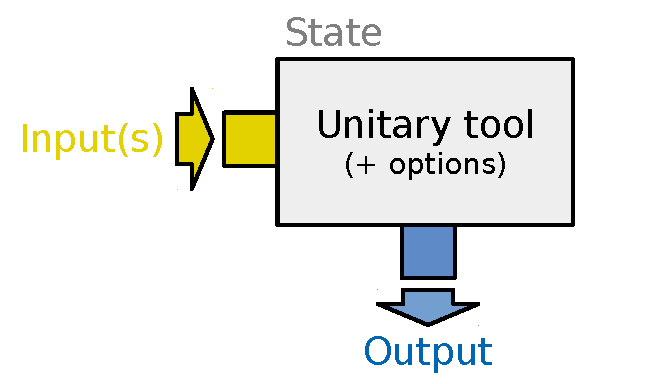
\includegraphics[width=0.4\textwidth]{schemas/PyTelTools_tool.pdf}

  \begin{columns}[onlytextwidth]
  \begin{column}{0.5\textwidth}
\begin{itemize}
    \item<1-> Each \textbf{unitary tool}:
      \begin{itemize}
      \item State {\tiny (Not configured, Ready, Sucess)}
      \item Options (configure)
      \item Input(s)/Output
      \end{itemize}
    \item<2-> \textbf{Combine them} in a \textbf{Directed Acyclic Graph} (DAG)
      \begin{itemize}
        \item data-type correctness
        \item junction
        \item data flows downward
        \item filters
        \item commutativity is sometimes possible (flexibility)
        \item<3> reproductability (project file)
        \item<3> reentrancy (intermediate files)
      \end{itemize}
\end{itemize}
  \end{column}
  \begin{column}{0.48\textwidth}
    \includegraphics<1>[width=0.8\textwidth]{schemas/PyTelTools_tool.pdf}\vspace{1cm}
    \includegraphics<1>[width=0.98\textwidth]{schemas/schema0.png}
    \includegraphics<2>[width=0.98\textwidth]{schemas/schema1bis.png}
    \includegraphics<3>[width=0.98\textwidth]{schemas/schema2.png}
  \end{column}
\end{columns}

\end{frame}


\subsection{Mono view}

\begin{frame}{Demo on Mono view}
  \centering
  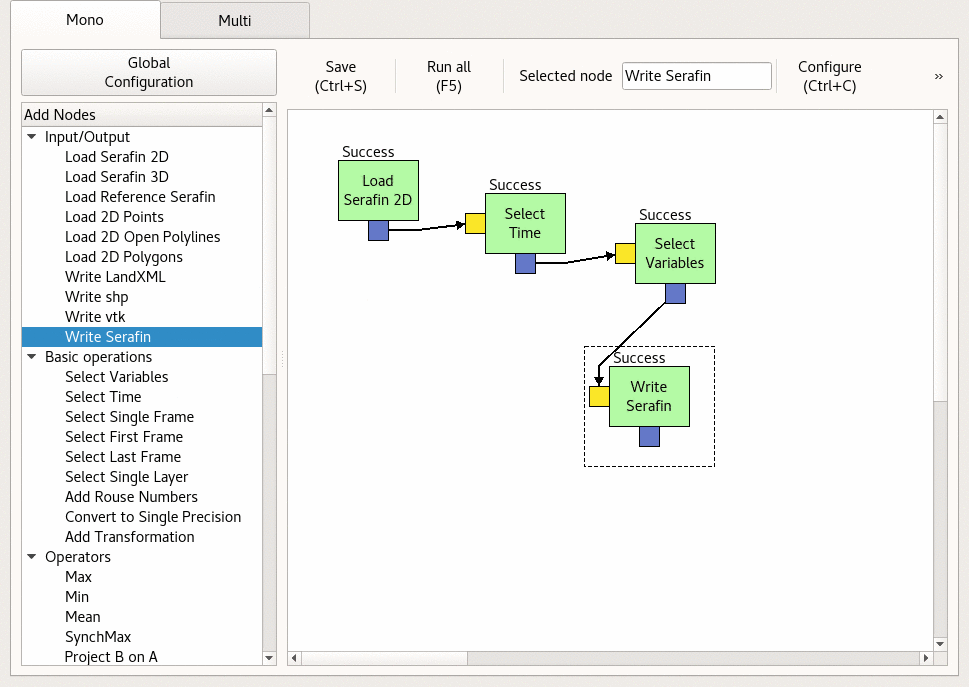
\includegraphics[height=7cm]{animation/mono_demo-430}
\end{frame}


\subsection{Multi view}

\begin{frame}{Repeat over multiple simulation}
  \begin{itemize}
    \item Prerequisites
    \begin{itemize}
      \item the graph is already configured
      \item input data are mostly identical and follows a naming convention
    \end{itemize}
    \item repeat over this serie of simulations
    \item parallelize on multiple CPU
    \item monitoring: status table, log events
  \end{itemize}
\end{frame}

\begin{frame}{Demo on Multi view}
  \centering
  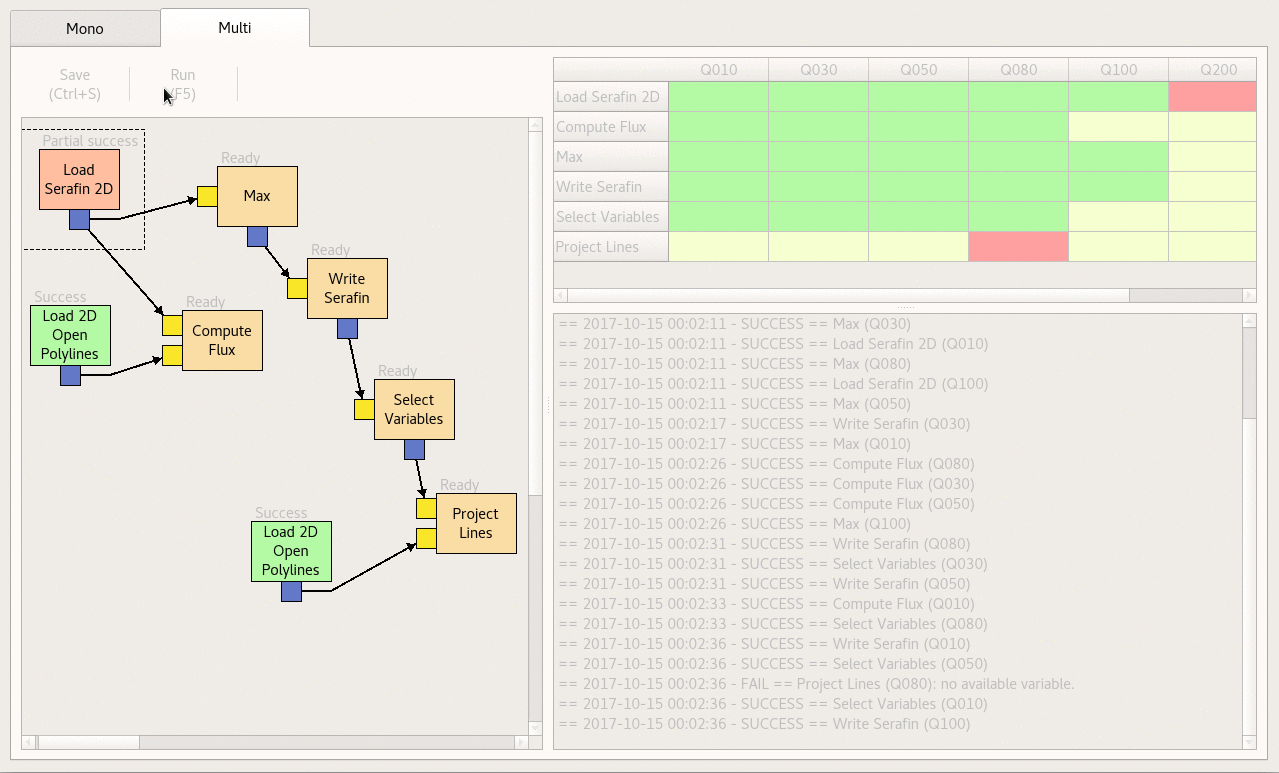
\includegraphics[height=7cm]{animation/multi_demo-181}
\end{frame}
